\chapter{Module Configuration Overview}
This chapter will describe some calibration and configuration parameters and helpful hints for configuring it.

\section{Configuration Parameters}

\subsection{SrvcMgr Containers}
\label{subsec:SrvcMgrContainer}

The SUM\_SrvcMgr provides a ParamDef file containing the following configuration parameters (Fig. \ref{fig:containerdiag}). This section will describe these parameters and their meaning.

\begin{figure}[H]
    \includegraphics[width=\textwidth,height=\textheight,keepaspectratio]{diagrams_generated/Sum_SrvcMgr_Containers.pdf}
    \caption{RTA-SUM SrvcMgr container diagram}
    \label{fig:containerdiag}
\end{figure}

\paragraph{Sum\_SrvcMgr\_General} Contains all the general configuration parameters that are common to all possible configurations for the module.
\begin{itemize}
  \item \textbf{Sum\_SrvcMgr\_PermitExecutionMask:} Mask used by SUM\_SrvcMgr in the Execution Manager to identify which bits of the PermitExecution Port Interface 
  shall be considered for triggering the start (RUN) or stop (SHUTDOWN) of its functions.
  \item \textbf{Sum\_SrvcMgr\_ExecutionManagerPeriodicity:} Period (ms) of the Execution Manager \\ Runnable. Runnable acting as SrcvMgr main function, handling internal modes and shutdown procedure.
  \item \textbf{Sum\_SrvcMgr\_GenerateInitRunnable} Is used to allow the generation of a periodic runnable to run function RE\_SrvcMgr\_Init one time. If TRUE the SrvcMgr generates the periodic runnable to execute init function one time otherwise, the init function is called by a BswM action list during startup.
  \item \textbf{Sum\_SrvcMgr\_InitFuncPeriodicity} Time in milliseconds, for the periodicity of the runnable init. Float values are supported. This parameter is required when \\Sum\_SrvcMgr\_GenerateInitRunnable is set to TRUE.
\end{itemize}


\paragraph{Sum\_SrvcMgr\_ConfigSet} Contains specific configuration sets according to SrvcMgr features and BswM dependencies.
\begin{itemize}
  \item \textbf{DCM References}
    \begin{itemize}
      \item \textbf{Sum\_SrvcMgr\_Did\_E0CC\_Ref:} Reference to DID 0xE0CC for retrieving the Learning Table Status.
      \item \textbf{Sum\_SrvcMgr\_Did\_E0CD\_Ref:} Reference to DID 0xE0CD for retrieving the Incomplete \\ Learning Table - Client section.
      \item \textbf{Sum\_SrvcMgr\_Did\_E0CE\_Ref:} Reference to DID 0xE0CE for retrieving the Incomplete \\ Learning Table - Server section.
      \item \textbf{Sum\_SrvcMgr\_Rid\_0654\_Ref:} Reference to RID 0x0654 configured in Dcm for triggering Service Learning Session.
      \item \textbf{Sum\_SrvcMgr\_Rid\_0612\_Ref:} Reference to RID 0x0612 configured in Dcm to retrieve the Learning Table content.
      \item \textbf{Sum\_SrvcMgr\_Sig\_PropSysActv\_Ref:} Com Signal reference for Propulsion System Active.
      \item \textbf{Sum\_SrvcMgr\_ServiceBased\_DataTypeMappingSet:} \texttt{DATA-TYPE-MAPPING-SET} reference for service-based operations (PSA and Vehicle Speed).
      \item \textbf{Sum\_SrvcMgr\_ServiceBased\_PropSysActv\_Ref:} \texttt{IMPLEMENTATION-DATA-TYPE-ELEMENT} reference for service-based PSA.
      \item \textbf{Sum\_SrvcMgr\_Sig\_VehSpdAvgDrvn\_Ref:} Com Signal reference for Vehicle Speed Average Driven.
      \item \textbf{Sum\_SrvcMgr\_ServiceBased\_VehSpdAvgDrvn\_Ref:} \texttt{IMPLEMENTATION-DATA-TYPE-ELEMENT} reference for service-based Vehicle Speed Average Driven.     
    \end{itemize}
\end{itemize}


\section{Configuration Hints}

\subsection{Initialization}
\label{subsec:initialization}
The SrvcMgr needs to be initialized before it can be used. 

If the \textit{Sum\_SrvcMgr\_GenerateInitRunnable} parameter is set to TRUE, the SrvcMgr will generate a periodic runnable to execute the internal init function. 
The user can configure the periodicity of the init runnable by setting the \textit{Sum\_SrvcMgr\_InitFuncPeriodicity} parameter. 


Otherwise, the \textit{Sum\_SrvcMgr\_Init} function shall configured in the BswM init action list to be called during the startup. 
In this case the function prototype is declared in the file \textit{Sum\_SrvcMgr.h} that shall be included in the BswM configuration.


\subsection{SrvcMgr Execution Manager}
\label{subsec:executionmask}
The SrvcMgr execution manager groups all that functionalities that:

\begin{enumerate}
    \item Check the external requests on the module;
    \item Set the module operating Mode;
    \item Produce the shutdown permission to the RTA-SUM SUSD; 
\end{enumerate}

\paragraph{Check the external requests}
The RTA-SUM SrvcMgr Execution Manager checks an external request coming from the \textbf{port}
\\RP\_SUSD\_SrvcMgr\_SUSD\_PermitExecution through the \textit{SUSD\_PermitExecution} \textbf{interface}.
\\The RTA-SUM SrvcMgr Execution Manager allows the execution of its submodules depending on the value received through this \textbf{interface} and the state of the request coming from the SPM.

\paragraph{Set module operating mode} The operating mode for the SrvcMgr is computed according the value read over the \textit{SUSD\_PermitExec ution} interface.
In order to move the modules to the running mode, it is necessary to configure bit masks that will filter the wished bits in \textit{SUSD\_PermitExecution}.\\
They shall be configured with \textbf{all don't care bits to 1 and 0s otherwise}.
The configurable bit mask is \code{Sum\_SrvcMgr\_PermitExecutionMask}.

The mode selection is done by a Finite State Machine. The Finite State Machine is periodically scheduled. The scheduling Periodicity can be 
set by the configuration parameter \\\code{Sum\_SrvcMgr\_ExecutionManagerPeriodicity}. The user \textbf{shall} configure this parameter in \textit{milliseconds}, in a range from 0 to 65535.0.
Please pay attention configuring this parameter: the SrvcMgr will not execute any releveant code until it moves to the running mode. 
\\It is strongly suggested to give a high priority to the task mapping this functionality OR assign a reasonable short periodicity. Since the SrvcMgr collects the information from the SUSD, the user shall be sure that 
the RTA-SUM SUSD has produced the request when they schedule the SrvcMgr Execution Manager.

\paragraph{Produce the shutdown permission}
After the execution of the internal Finite State Machine, the SrvcMgr produces the value of the shutdown permission on the port implementing the 
\textit{SrvcMgr\_ShutdownPermission} interface. Please make sure to connect it to the RTA-SUM SUSD in order to grant the correct management of the system execution and requests handling.

\paragraph{Interaction with SSFM module for setting DTCs}
For SSFM module to be able to set DTC U19A6 87, during the execution of the SrvcMgr Execution Manager, the following port needs to be connected:
 \begin{itemize}
    \item PP\_SrvcMgr\_SSFM\_LearningTableStatus to SSFM
  \end{itemize}
In addition, the user shall connect the PP\_SrvcMgr\_SSFM\_U19A6\_57\_Status and PP\_SrvcMgr\_Errh\_\\U19A6\_54\_Status to the SSFM module to set or reset the corresponding DTCs.

\textbf{Note: Actions related to DTCs are only performed if battery voltage is available and only once.} 

\subsection{SrvcMgr Learning Session Manager}
The SrvcMgr Learning Session Manager groups the functions supporting the RIDs and DIDs related to the Service Learning Session. This section provides a guideline about the configuration and 
connections expected by SUM\_SrvcMgr Learning Session Manager.

The integrator must include references to the DIDs and RIDs configured in the DCM, as explained in the \ref{sec:DcmConf} section.
\begin{figure}[H]
	\centering
	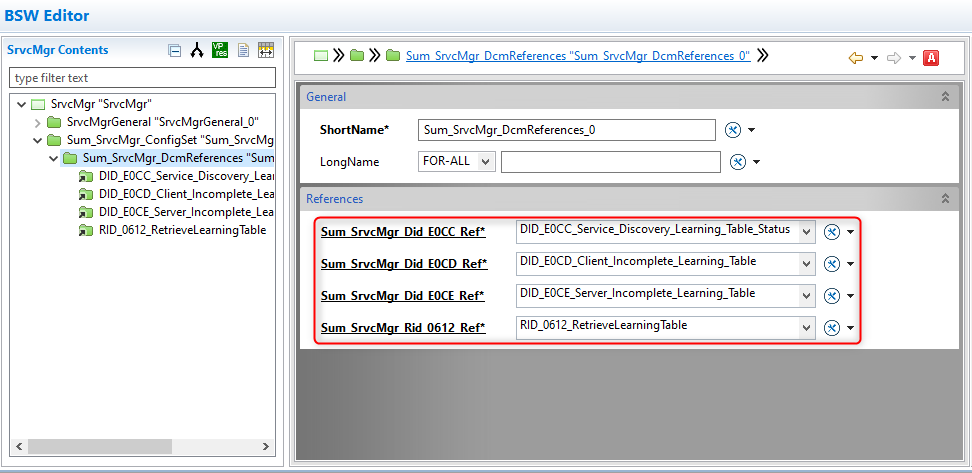
\includegraphics[scale=0.55]{images/SumSrvcMgrDcmReferences.png}
\end{figure} 

\subsubsection{DID 0xE0CC}
DID 0xE0CC is used to provide the status of the Learning Table.
\\Is necessary to configure the DID in Dcm as specified in the \ref{sec:DcmConf0xE0CC} section in order to obtain a result as expected.

Please connect the port related to the DID 0xE0CC \\ (PP\_SrvcMgr\_DCM\_DID\_E0CC\_$<$dcmDspDidSignal\_shortname$>$) to Dcm.

\subsubsection{DID 0xE0CD and DID 0xE0CE}
\label{subsec:DIDsE0CDandE0CE}
DID 0xE0CD is used to provide the list of services expected to be learnt but were not found/discovered. It also maintains a buffer to track the services that are missing from SSFM.
\\Connect the port interface SSFM\_SrvcMgr\_SDMissingMessage from SSFM to SrvcMgr to obtain the missed services.
\\DID 0xE0CE is used to provide the list of services expected to be subscribed to but were not acknowledged.
\\Is necessary to configure both DIDs as specified in the \ref{sec:DcmConf0xE0CD} section in order to obtain a result as expected.

\subsubsection{RID 0x0654}
\label{subsec:RID0x0654}
RID responsible for triggering the Learning Session.

It is necessary to configure the RID in the Dcm module as specified in the \ref{sec:RID0654} section in order to obtain the expected result.

The DCM\_E\_GENERALREJECT NRC is retrieved if the API Sd\_ClearLearningTable returns \\ E\_NOT\_OK.
If the conditions above occurs, the Runnable associated with the RID will return E\_NOT\_OK.

Moreover, connect the following SrvcMgr port related to RID 0x0654 to Dcm module respectively:
 \begin{itemize}
    \item PP\_SrvcMgr\_Dcm\_RID\_0654\_TriggerLearningSession to Dcm
  \end{itemize}

For the interactions with SSFM module, during the execution of the RID 0x0654, the following ports need to be connected:
 \begin{itemize}
    \item PP\_SrvcMgr\_SSFM\_LearningTableStatus to allow the SSFM module to set DTC U19A6 87 at the end of RID 0x0654 execution.
    \item PP\_SrvcMgr\_SSFM\_U19A6\_57\_Status and PP\_SrvcMgr\_Errh\_U19A6\_54\_Status to set or reset the corresponding DTCs.
  \end{itemize}

Additionally, for RID 0x0654 enable condition checking, the SSFM fault-status ports shall be connected according to the SSFM and signal-reference configuration:
 \begin{itemize}
    \item If \texttt{Sum\_Ssfm\_FxI\_FxFA\_SinglePortsSupport = TRUE} and VSAD/PSA share the same signal/service reference: connect RP\_SSFM\_SrvcMgr\_FxFA\_VSAD\_PSA.
    \item If \texttt{Sum\_Ssfm\_FxI\_FxFA\_SinglePortsSupport = TRUE} and VSAD/PSA use different references: connect RP\_SSFM\_SrvcMgr\_FxFA\_VSAD and RP\_SSFM\_SrvcMgr\_FxFA\_PSA.
    \item If \texttt{Sum\_Ssfm\_FxI\_FxFA\_SinglePortsSupport = FALSE} and VSAD/PSA share the same signal/service reference: connect RP\_SSFM\_SrvcMgr\_FsFA\_VSAD\_PSA.
    \item If \texttt{Sum\_Ssfm\_FxI\_FxFA\_SinglePortsSupport = FALSE} and VSAD/PSA use different references: connect RP\_SSFM\_SrvcMgr\_FsFA\_VSAD and RP\_SSFM\_SrvcMgr\_FsFA\_PSA.
  \end{itemize}


\subsubsection{RID 0x0612}
\label{subsec:RIDs0x0612}
RID responsible to retrieve the Learning table content. The content provided by SrvcMgr when this RID is requested is function of the Control Option received as specified in the SDV-6001:
\begin{itemize}
\item Number of Client Service Ids or Server Service Ids learned;
\item Range of Client Service Ids or Server Service Ids learned;
\end{itemize}

It is necessary to configure the RID as specified in the \ref{sec:DcmConf0x0612} section in order to obtain a result as expected. 

You need to pay attention that the SrvcMgr makes check over the consistency of the Control Option received retrieving a NRC if necessary:
\begin{itemize}
\item DCM\_E\_CONDITIONSNOTCORRECT: if one of the following scenarios occurs:
		\begin{itemize}
		\item if the Control Option \#1 is not consistent with the Control Option \#2 as specified in SDV-6001 document (i.e. Control Option \#1 0x00 and Control Option \#2 0x00); 
		\item if Start\_of\_Range is greater than End\_of\_Range (specified in Control Option \#3);
		\item if the Control Option \#3 is not zero when the first two Control Options request to retrieve the number of instance of Services;
		\item if the Propulsion System Active signal is not FALSE (enable condition for RID execution);
		\end{itemize}
\end{itemize}

The DCM\_E\_GENERALREJECT NRC is retrieved if the API Sd\_RetrieveLearnigTable return E\_NOT\_OK.
\\If one of the condition above occours, the Runnable associated to the RID will return E\_NOT\_OK. 


If the range of Service Ids is requested (Control Option\#1 0x00), the range of Control Option\#3 is:
\begin{itemize}
  \item Start of range (2 Byte): the lowest value of service IDs to retrieve.
  \item End of range (2 Byte): the highest value of service IDs to retrieve.
  \end{itemize}

Moreover, it is required to connect the port related to the RID0x0612 (PP\_SrvcMgr\_Dcm\_RID\_0612) to Dcm.

\subsubsection{Propulsion System Active Flag Configuration}
\label{sec:propsysactflag}
SUM\_SrvcMgr supports both signal-based and service-based configurations for Propulsion System Active signal.

SUM\_SrvcMgr needs to read and evaluate the Propulsion System Active signal as an enable condition for RID 0x0612 (Retrieve Learning Table).
To do that, it reads the value of \textit{PropSysActv} signal via the RTE port interface RP\_Com\_SrvcMgr\_VePSAR\_b\_PropSysActv.
RID 0x0612 will only execute when the Propulsion System Active signal is FALSE, ensuring that learning table retrieval operations are only performed when the propulsion system is not active.

For this purpose, the signal must be referenced in the Sum\_SrvcMgr\_PropSysActv\_Ref parameter.

\subsubsection{Service-Based PropSysActv Configuration}
\label{sec:servicebasedpropsysactv}
For service-based PropSysActv operations, SUM\_SrvcMgr requires additional configuration to properly reference the system data type mappings and implementation data type elements. The following parameters enable this functionality:

\textbf{Sum\_SrvcMgr\_Sig\_PropSysActv\_Ref Configuration:}

This choice reference parameter configures the reference to the Com Signal for Propulsion System Active. The signal can be configured as either:
\begin{itemize}
  \item Service Based (ComSignal)
	\item Signal Based (ComSignal)
	\item Signal Based (ComGroupSignal)
\end{itemize}

\textbf{Sum\_SrvcMgr\_ServiceBased\_DataTypeMappingSet Configuration:}

This foreign choice reference parameter configures the reference to the DATA-TYPE-MAPPING-SET in the system extract. The parameter must be configured to point to the correct data type mapping set used for service-based operations including PropSysActv and Vehicle Speed. This parameter supports multiple references (UPPER-MULTIPLICITY-INFINITE) to accommodate different data type mapping sets for various service-based functionalities.

\textbf{Sum\_SrvcMgr\_ServiceBased\_PropSysActv\_Ref Configuration:}

This foreign reference must be configured to the specific IMPLEMENTATION-DATA-TYPE-ELEMENT that contains the service-based PropSysActv functionality within the software architecture packages. This reference establishes the connection between the SrvcMgr module and the system's PropSysActv implementation data types.

\begin{figure}[H]
	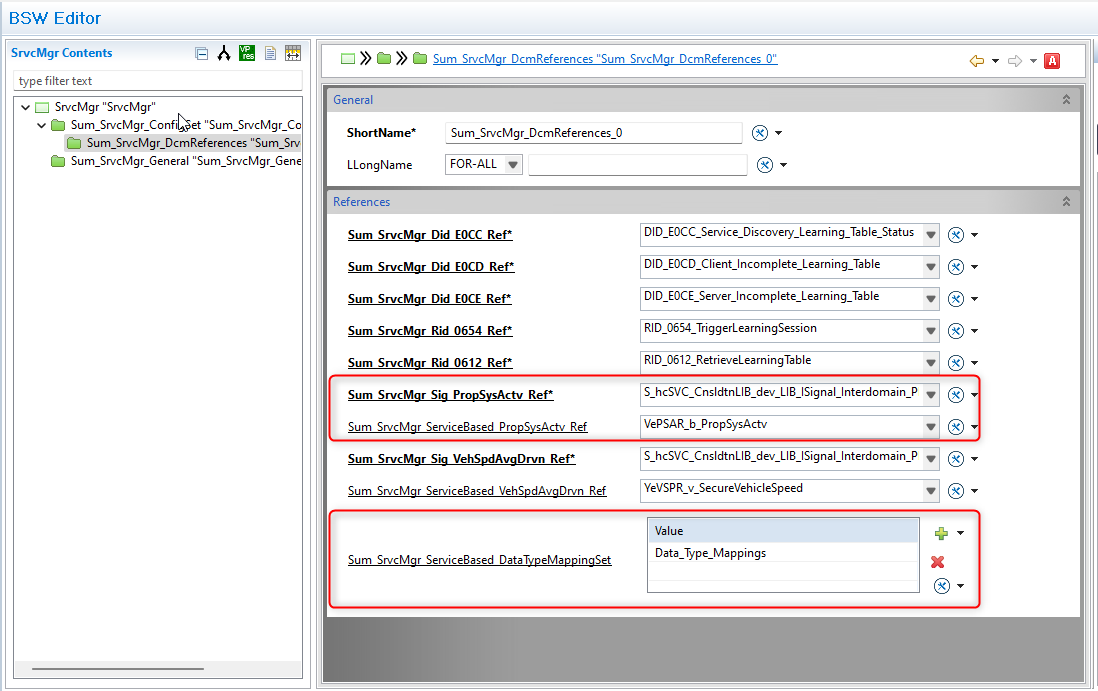
\includegraphics[width=1\textwidth]{images/RID_0x0612_PropSysActv.png}
	\caption{ RTA-SUM SrvcMgr Service-Based PropSysActv}
\end{figure}

\textbf{Configuration Dependencies:}
When configuring service-based PropSysActv operations, ensure that:
\begin{itemize}
	\item The \texttt{Sum\_SrvcMgr\_ServiceBased\_DataTypeMappingSet} references a valid DATA-TYPE-MAPPING-SET in the system extract
	\item The \texttt{Sum\_SrvcMgr\_ServiceBased\_PropSysActv\_Ref} references an existing IMPLEMENTATION-DATA-TYPE-ELEMENT
	\item The referenced implementation data type element is properly defined in the system architecture
	\item The data type mappings are consistent with the system's service-based PropSysActv implementation
	\item The port RP\_Com\_SrvcMgr\_VePSAR\_b\_PropSysActv is properly connected to the Com module for receiving the PropSysActv signal by mapping 
\end{itemize}

\subsubsection{Vehicle Speed Average Driven Configuration}
\label{sec:vehspdavgdrvn}
SUM\_SrvcMgr supports both signal-based and service-based configurations for Vehicle Speed Average Driven signal.

SUM\_SrvcMgr needs to read and evaluate the Vehicle Speed Average Driven signal for vehicle speed related operations, particularly for RID 0x0612 (Retrieve Learning Table) and RID 0x0654 (Service Discovery Learning Session).

It reads the value of \textit{VehSpdAvgDrvn} via the port interface RP\_Com\_SrvcMgr\_YeVSPR\_v\_DrvnVehicle.

For this purpose, the signal must be referenced in the Sum\_SrvcMgr\_Sig\_VehSpdAvgDrvn\_Ref parameter.

\textbf{Sum\_SrvcMgr\_Sig\_VehSpdAvgDrvn\_Ref Configuration:}

This choice reference parameter configures the reference to the Com Signal for Vehicle Speed Average Driven. The signal can be configured as either:
\begin{itemize}
  \item Service Based (ComSignal)
	\item Signal Based (ComSignal)
	\item Signal Based (ComGroupSignal)
\end{itemize}

The SrvcMgr module reads this signal via the RTE port interface to obtain vehicle speed information for various operations.

\textbf{Sum\_SrvcMgr\_ServiceBased\_VehSpdAvgDrvn\_Ref Configuration:}

This foreign reference must be configured to the specific IMPLEMENTATION-DATA-TYPE-ELEMENT that contains the service-based Vehicle Speed Average Driven functionality within the software architecture packages from the System Extract. This reference enables service-oriented communication for vehicle speed data.

\begin{figure}[H]
	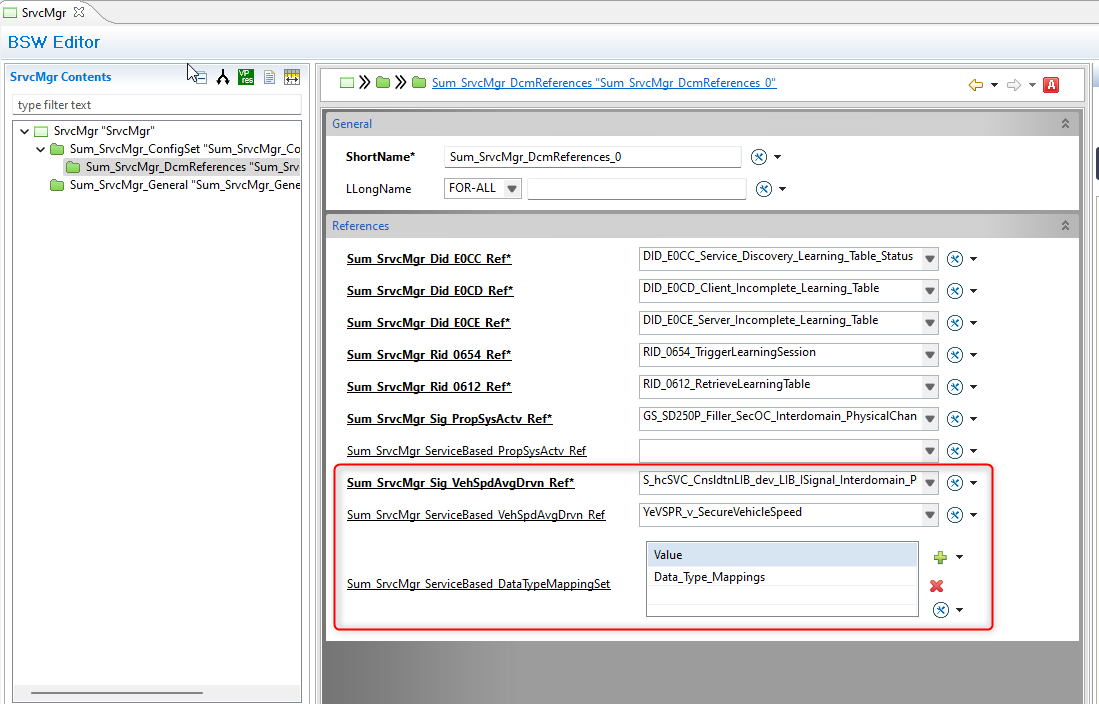
\includegraphics[width=1\textwidth]{images/RID_0x0612_RID_0x0654_VehSpdAvgDrvn.png}
	\caption{ RTA-SUM SrvcMgr Service-Based VehSpdAvgDrvn}
\end{figure}

\textbf{Configuration Dependencies:}
When configuring Vehicle Speed Average Driven operations, ensure that:
\begin{itemize}
	\item The \texttt{Sum\_SrvcMgr\_Sig\_VehSpdAvgDrvn\_Ref} references a valid ComSignal or ComGroupSignal
	\item The \texttt{Sum\_SrvcMgr\_ServiceBased\_VehSpdAvgDrvn\_Ref} references an IMPLEMENTATION-DATA-TYPE-ELEMENT (when using service-based communication)
	\item The \texttt{Sum\_SrvcMgr\_ServiceBased\_DataTypeMappingSet} includes appropriate data type mapping sets for vehicle speed operations
	\item The referenced implementation data type element is properly defined in the system architecture
	\item The Com signal is properly connected to the SrvcMgr required port interface before RTE code generation
\end{itemize}

\textbf{Note - Unified Configuration for Service-Based PSA and Vehicle Speed:} 

The \texttt{Sum\_SrvcMgr\_ServiceBased\_DataTypeMappingSet} parameter is used for both Propulsion System Active (PSA) and Vehicle Speed Average Driven service-based configurations. This unified data type mapping set enables consistent service-based communication for both signal types across the module. 

Additionally, when both PSA and Vehicle Speed Average Driven are provided as service-based signals, the SrvcMgr module can utilize the unified port interface \textit{RP\_Com\_SrvcMgr\_VeActvProp\_YeDrvnVeh} to access both signals through a single interface, providing simplified configuration and unified access for RID 0x0612 (Retrieve Learning Table) and RID 0x0654 (Trigger Learning Session) enable condition checking.

\textbf{Signal Configuration Summary} 

\begin{table}[H]
\centering
\begin{tabular}{|l|l|l|l|}
\hline
\textbf{Signal} & \textbf{Mode} & \textbf{Category} & \textbf{Type} \\ \hline
\multirow{3}{*}{PropSysActv} & Service-Based & ComSignal & UINT8\_N \\ \cline{2-4} 
 & Signal-Based & ComSignal/ComGroupSignal & UINT8/BOOLEAN \\ \hline
\multirow{3}{*}{VehSpdAvgDrvn} & Service-Based & ComSignal & UINT8\_N \\ \cline{2-4} 
 & Signal-Based & ComSignal/ComGroupSignal & FLOAT32 \\ \hline
\end{tabular}
\caption{Valid Signal Configurations}
\label{tab:signalconfigs}
\end{table}

\textbf{Key Rules:}
\begin{itemize}
	\item Service-based \textbf{requires} ComSignal with UINT8\_N (ComGroupSignal not allowed)
	\item Signal-based allows ComSignal or ComGroupSignal with fixed-size types
\end{itemize}


\subsection{ServiceManager}
\label{SrvcMgr}

This section provides a guideline about the usage of the API configured in the Service Manager.

\subsubsection{API SrvcMgr\_ActivateServices}
This API is used to set a specific state for a list of Service ID. The result of these operations are retrieved to the caller of the API in the commandStatusList.
The number of Service ID (length of serviceIdList) must be specified in the listLength by the caller of the API and must match with the length of the 
activationCommandList and commandStatusList. 
The same index for each of these three arrays correspond a Service ID on which we want to set a specific state and the result in retrieved in the same index
of the commandStatusList.

Each member of the array activationCommandList can assume just two value (TRUE or FALSE):
\begin{itemize}
\item TRUE: to set a Server Service to SD\_SERVER\_SERVICE\_AVAILABLE or a Client Service SD\_CLIENT\_ SERVICE\_REQUESTED (unformally to enable a Service);
\item FALSE: to set a Server Service to SD\_SERVER\_SERVICE\_DOWN or a Client Service SD\_CLIENT\_ SERVICE\_RELEASED (unformally to disable a Service); 
\end{itemize}
Please note that this API selects the Sd API based on the Service Group configuration. If the service belongs to a Service Group, SrvcMgr uses Sd\_ServiceGroupStart()/Sd\_ServiceGroupStop() and does not call Sd\_ServerServiceSetState() or Sd\_ClientServiceSetState(). If the service does not belong to a Service Group, SrvcMgr uses Sd\_ServerServiceSetState() for server services and Sd\_ClientServiceSetState() for client services.
For non-group services, the activation helper distinguishes client vs server instances, maps the activation flag to Sd\_ClientServiceSetState() or Sd\_ServerServiceSetState(), and records E\_OK\_REMOTE\_ENABLED or E\_OK\_LOCAL\_ENABLED on success. When a requested client service owns consumed event groups, Sd\_ConsumedEventGroupSetState() is called for each configured group; any E\_NOT\_OK moves the related status to E\_GENERAL\_ERROR. Sum\_Srvcmgr\_SetClientSrvcRequestedRemoteSrvcAvailable() reuses the same helper so that bulk client requests follow the same Service Group vs non-group rules.
Refer to the Sd module specification to understand more deeply the meaning of SD\_SERVER\_SERVICE\_AVAILABLE, SD\_CLIENT\_SERVICE\_REQUESTED, SD\_SERVER\_ SERVICE\_DOWN and SD\_CLIENT\_SERVICE\_RELEASED.


Each member of the array commandStatusList can assume the following value:
\begin{itemize}
\item E\_OK\_LOCAL\_ENABLED (0x00): Service is calibrated On and is a local service (Sd Server Service); 
\item E\_OK\_REMOTE\_ENABLED (0x01): Service is calibrated On and is a remote service (Sd Client Service);
\item E\_DISABLED (0x02): Service is calibrated Off and is local or remote Service (Sd Server or Sd Client Service);
\item E\_GENERAL\_ERROR (0x03): Service not configured or the SD APIs used returns E\_NOT\_OK for that particular Server or Client Service; 
\end{itemize}

Moreover, this API is triggered by the C/S interface SrvcMgr\_SPM\_ActivateServices.


\subsection{Calibration Controller}
\label{CalContr}

This section provides guidelines about the usage of the APIs configured in the Calibration Controller.

\subsubsection{Initialization}
Please remember to connect the client-server interface SrvcMgr\_CalibrationController to properly allow the calibration of the services and service groups.

\subsubsection{Runnable\_SrvcMgr\_DisableService}
SUM\_SrvcMgr implements the Runnable\_SrvcMgr\_DisableService that will be called through the C/S interface SrvcMgr\_ServiceCalibrationOff (operation SrvcMgr\_DisableService) 
by the SWCs to change the state (disable) of services through SD APIs.

This Runnable take as input parameter the ID value of the Service that the user want to disable. 

Please, take into account that ID refer to the SdClientServiceId or SdServerServiceId specified in the container Sd/SdConfig/SdInstance/SdClientService for a Client Service or 
Sd/SdConfig/SdInstance/SdServerService for a Service Service. The Runnable Runnable\_SrvcMgr\_DisableService understand by itself if the ID received correspond to a Client or Server Service.

This Runnable will change the status of a Service through SD APIs:

\begin{itemize}
\item Call to Sd\_ServerServiceSetState()/Sd\_ClientServiceSetState();
\item Call to Sd\_CalibrateServicesOff();
\end{itemize}

The Runnable\_SrvcMgr\_DisableService return the following value: 
\begin{itemize}
\item E\_OK: if the Service is properly disabled.
\item E\_NOT\_OK: if the Service is NOT properly disabled for the following reason:
\begin{itemize}
\item The Service ID is not configured in the SD container; 
\item One of the SD APIs called return E\_NOT\_OK;
\end{itemize}
\end{itemize}

Please, refer to the SD module specification in order to understand the meaning of possible E\_NOT\_OK received by the SD APIs. 
The user SHALL connect the port PP\_SrvcMgr\_ServiceCalibrationOff to their SWC and configure the call in synchronous way in order to trigger this Runnable properly.

\subsubsection{Runnable\_SrvcMgr\_DisableServiceGroup}
SUM\_SrvcMgr implements the Runnable\_SrvcMgr\_DisableServiceGroup that will be called through the C/S interface SrvcMgr\_ServiceCalibrationOff (operation SrvcMgr\_DisableServiceGroup) 
by the SWCs to change the state (disable) of services group through SD APIs.

This Runnable takes, as an input parameter, the ID value of the Group Service that the user wants to disable. 

Please, take into account that ID refer to the SdServiceGroupHandleId specified in the container Sd/SdConfig/SdServiceGroup.

This Runnable will change the status of a Group Service through SD APIs:

\begin{itemize}
\item Call to Sd\_ServiceGroupStop();
\item Call to Sd\_CalibrateServicesOff();
\end{itemize}

The Runnable\_SrvcMgr\_DisableServiceGroup return the following value: 
\begin{itemize}
\item E\_OK: The Service Group is properly disabled.
\item E\_NOT\_OK: if the Service Group is NOT properly disabled for the following reason:
\begin{itemize}
\item There is no Service Group configured in the SD container; 
\item The Service Group ID is not configured in the SD container; 
\item The Service Group does not have at least one service associated; 
\item The API Sd\_CalibrateServicesOff() returns E\_NOT\_OK;
\end{itemize}
\end{itemize}

Please, refer to the SD module specification in order to understand the meaning of possible E\_NOT\_OK received by the SD API.\\
The user SHALL connect the port PP\_SrvcMgr\_ServiceCalibrationOff to their SWC and configure the call in synchronous way in order to trigger this Runnable properly.\\
Moreover, the integrator SHOULD follow the normal workflow about the generation: firstly generate the BSW and then the SrvcMgr. This is necessary since the Sd/SdConfig/SdServiceGroup/SdServiceGroupHandleId parameter
is a forwarded value: the integrator SHALL not put a value there because it is already done during the BSW generation by itself. 

